\subsection{Android Studio}
Both the smartphone application as well as the Google Glass application was developed in Android Studio~\cite{androidStudio}. Android Studio is a development environment developed by Google. %[TODO why Android Studio]

\subsection{ZXing}
The application was built upon the open-source barcode image processing library, Zebra Crossing (ZXing)~\cite{zxing}. %[TODO Vilka förändringar har gjorts]
% https://github.com/zxing/zxing/

\subsubsection{BarcodeEye}
The Google Glass application was built upon the Google Glass port of the ZXing library, known as BarcodeEye~\cite{barcodeEye}.% [TODO vilka förändringar har gjorts]%While a slideview was implemented in BarcodeEye already, the information displayed was static [todo, var den statisk]. The slideview consited of only two slides [todo code example of how it was static]. Mixing images with text was not possible either. Information also had to be encoded directly into the QR code and could not be downloaded by an encoded link.
% https://github.com/BarcodeEye/BarcodeEye

\subsection{View Slider}


\subsection{AsyncTask}
%Used for image, as well as product


\subsection{Text Split}


\subsection{Card Layout}
%which standard layout were used, one non-standard


\subsection{Test Cases}
%The following section describes how the tests were set up and carried out.
%
%\subsubsection{Experimental Setup}
The tests were carried out using an optical bench to guarantee scientific accuracy. The experimental setup contained an optical bench, with a screen holder at the zero point, where the QR code was positioned. The device being tested, Google Glass or smartphone, was then positioned at the specified mark on the optical bench using a clamp and pointed towards the QR code. See Figure~\ref{experimentalSetup} for a better understanding of the experimental setup. 

As seen in Figure~\ref{experimentalSetup} Google Glass was mounted in such a way that the camera sat a bit closer to the QR code than where the clamp marked on the optical bench. In order to compensate for the slight misalignment the clamp was positioned a few centimeters back from the specified mark and as such not used to determine the distance to the QR code. Instead the camera on Google Glass was used to pinpoint the exact distance to the QR code, and the clamp was positioned in such a way that the camera on Google Glass was at the distance specified in each experiment. In other words, even though the clamp was not at the same distance to the QR code for the smartphone tests as for the Google Glass tests, the camera of each device was.

	\begin{figure}[H]%ht!]
		\centering
    		\subfloat[The experimental setup for Google Glass.]{{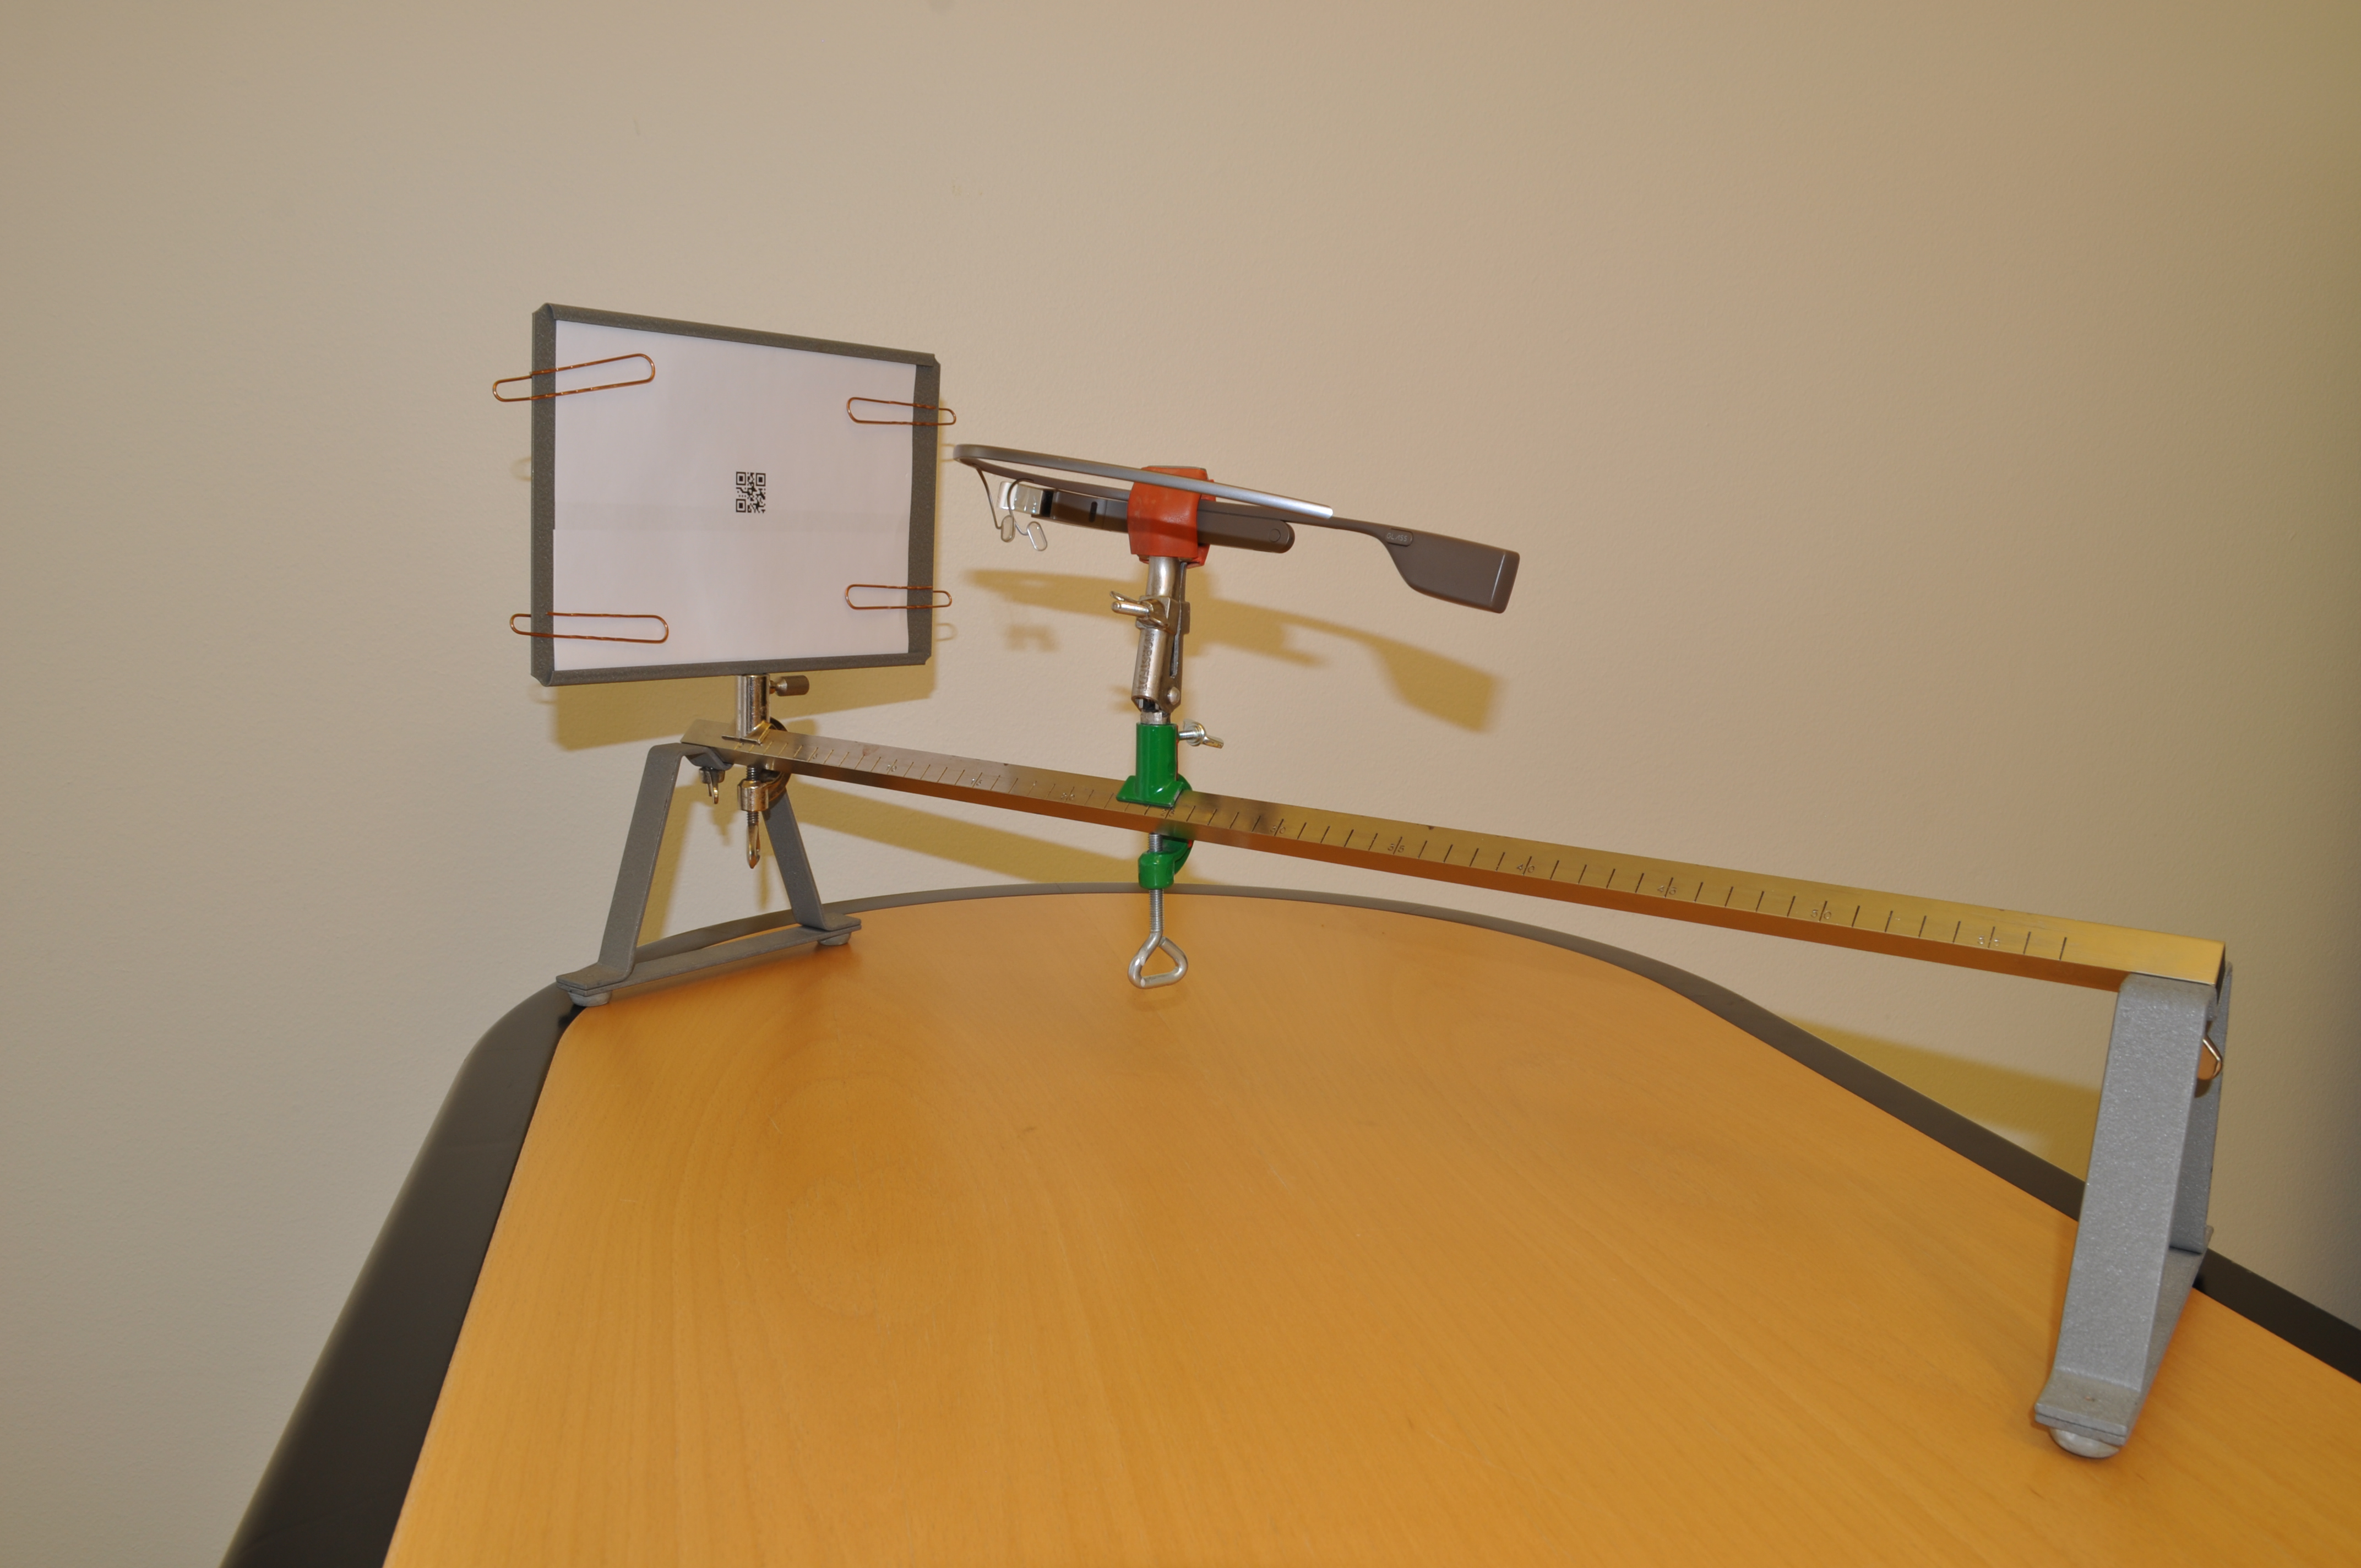
\includegraphics[width=70mm]{images/testSetupGlass}}}
   		 \qquad
		\subfloat[The experimental setup for Samsung Galaxy SII.]{{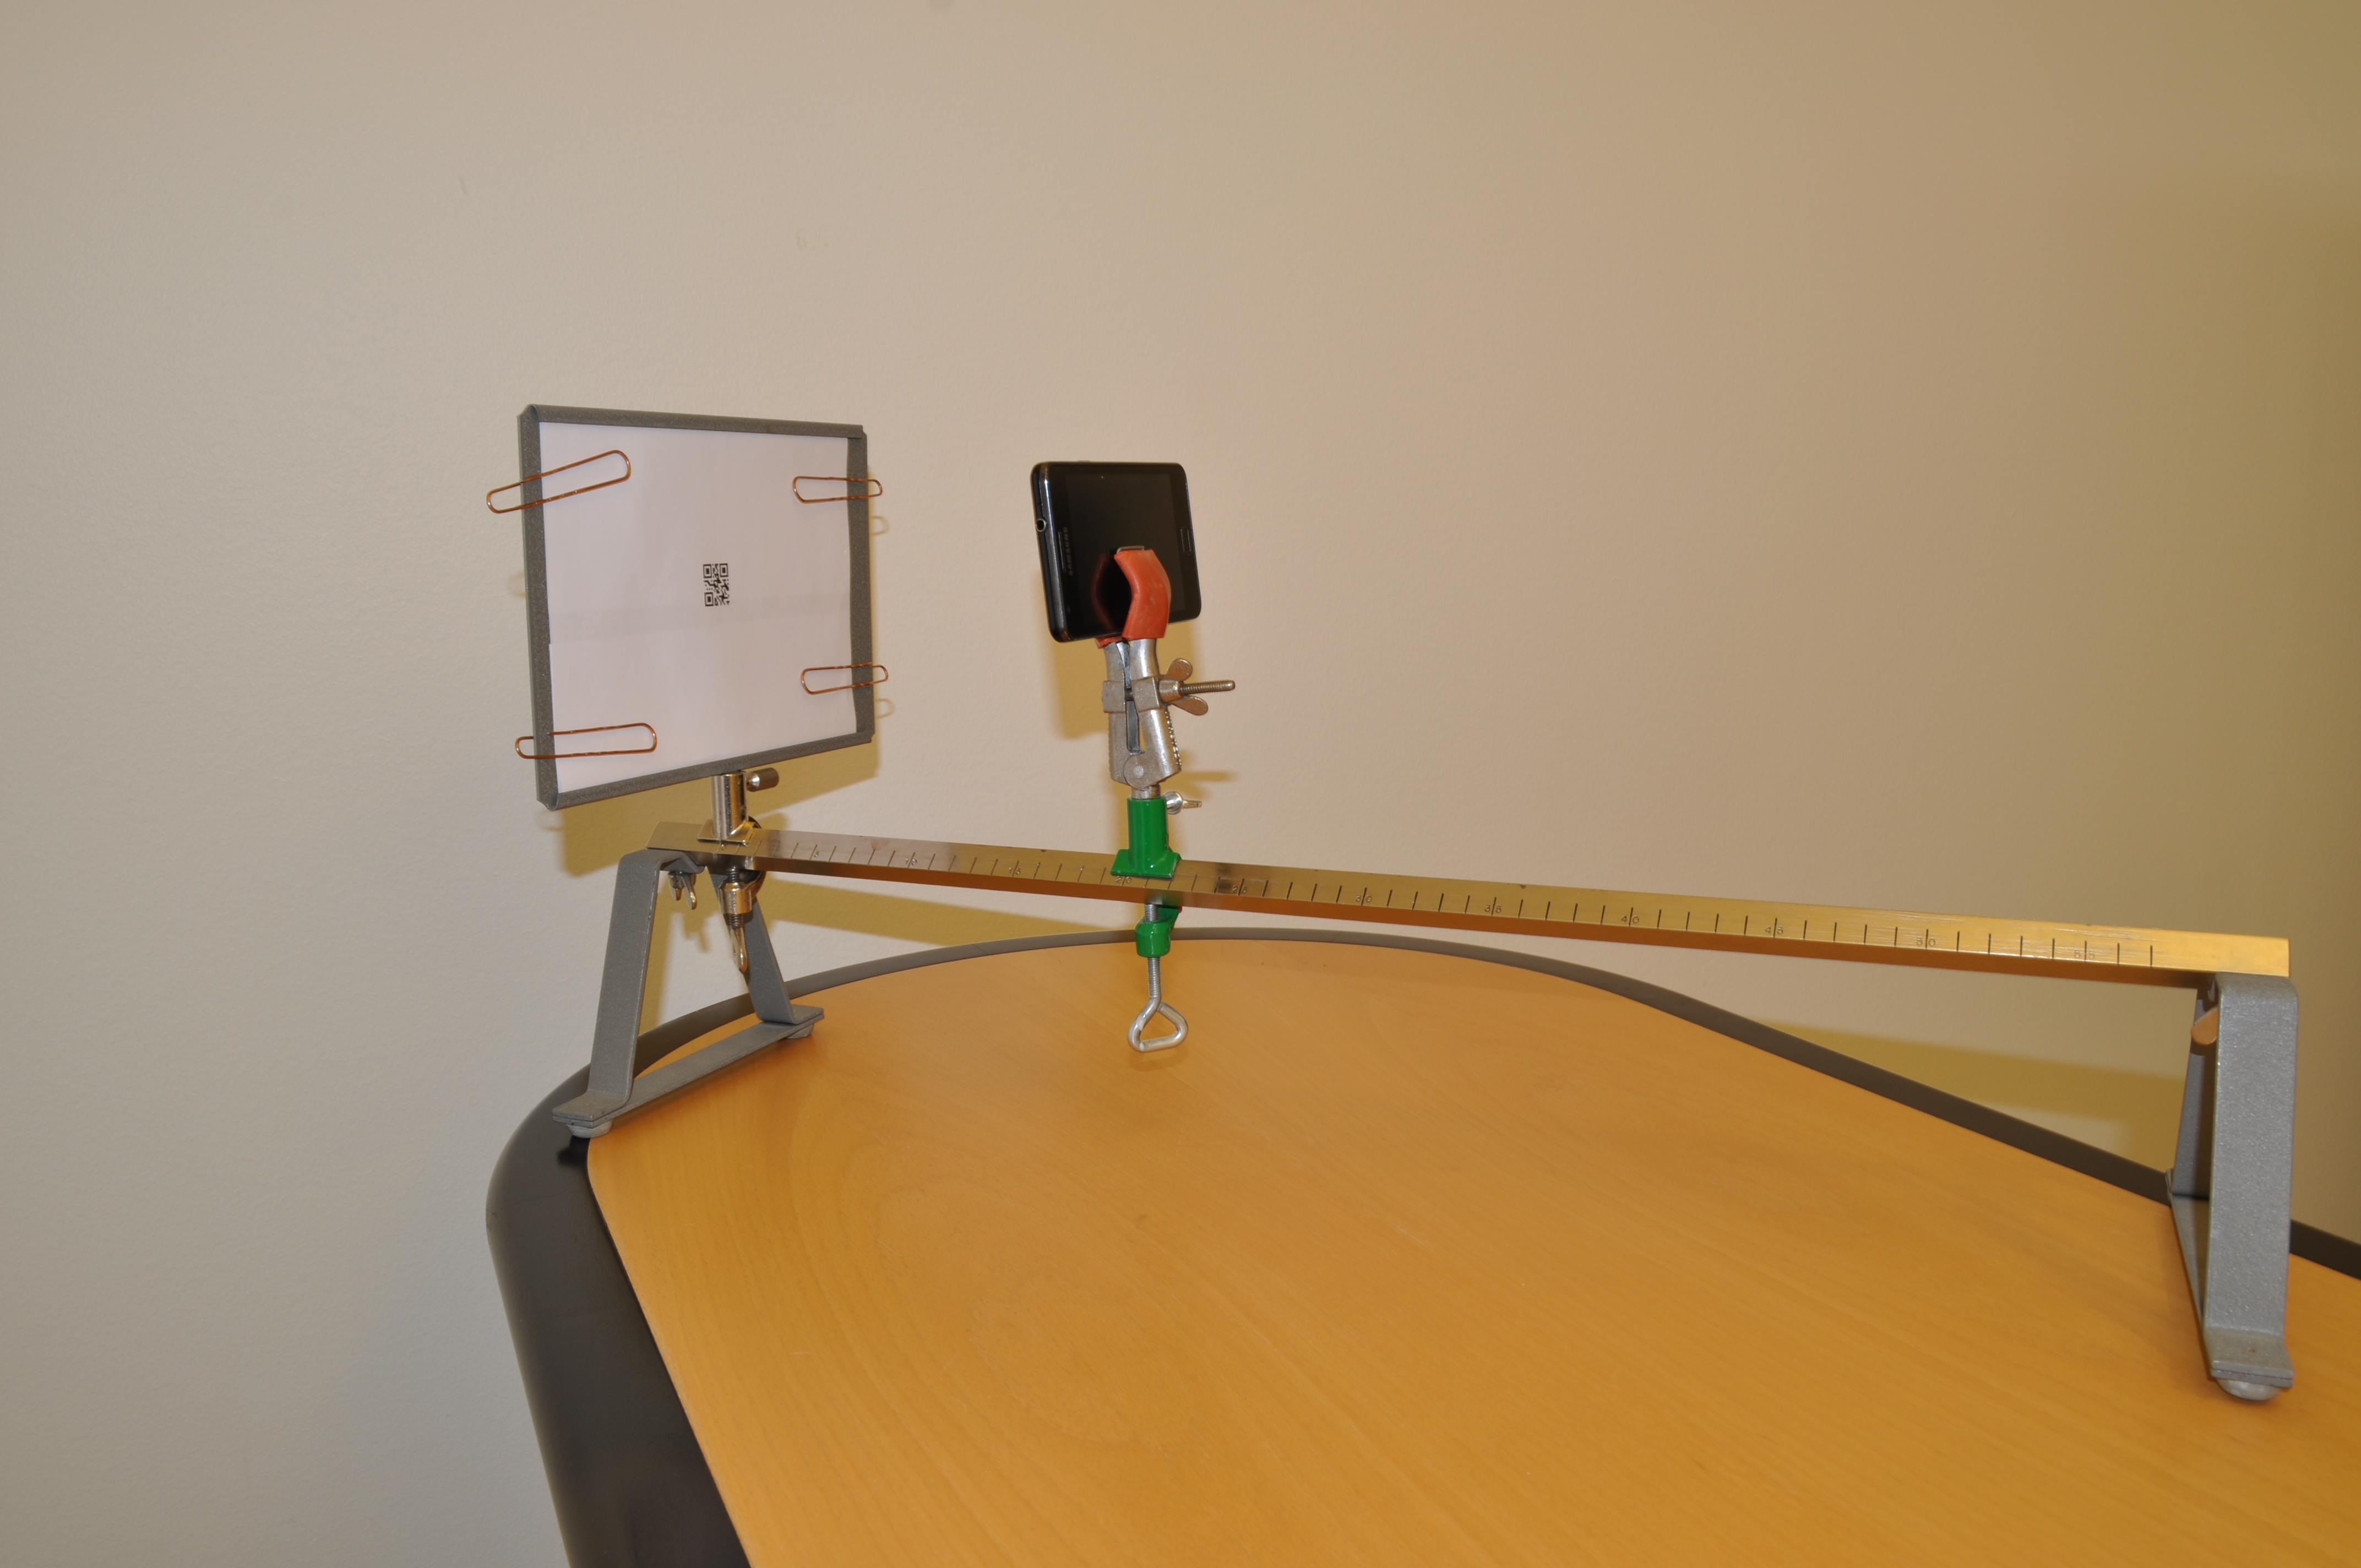
\includegraphics[width=70mm]{images/testSetupS2}}}
   		 \qquad
		\caption{The experimental setup.}
		\label{experimentalSetup}
	\end{figure}

Although not shown i Figure~\ref{experimentalSetup} each device was connected to a computer via a USB cable. The result time of each test was obtained from the log within Android Studio after each run, since when running an android application via Android Studio, log information may be obtained through the log within Android Studio.

In order to measure the time needed for the results of each test a specific class was built, called \texttt{Timer} (seen in Listing~\ref{timerClass}). The \texttt{Timer} class was built using the singleton design pattern. A singleton class is a class that can only be instanced once during the entire execution of an application. However the instance of a singleton class lives throughout the entire execution and may be accessed from anywhere in the application.

Using the singleton pattern meant that the timer could be started in one class, and stopped in another without having to pass the instance around, which could potentially affect the performance of each device.

\begin{lstlisting}[language=Java, caption={The Timer class}, label=timerClass]

public class Timer {
	private static Timer ourInstance = new Timer();
	public static Timer getInstance() { return ourInstance; }
	private Timer() {  }
	
	private boolean timerRunning = false;
	private Long startTime;
	private Long stopTime;
	
	public void startTimer() { 
		if(timerRunning) { Log.d("TIMER", "Timer already running"); }
		else 	{ startIme = System.nanoTime(); }
	}
	
	public void stopTimer() {
		if(!timerRunning) { Log.d("TIMER", "No timer running"); }
		else { stopTime = System.nanoTime()); }
	}
	
	private long getElapsedTime(int timerID) { return stopTime - startTime; }
	
	public void logElapsedTime(String information) {
		Log.d("TIMER", information + ": " + String.valueOf(getElapsedTime() + " nano seconds");
	}
}
\end{lstlisting}

\subsubsection{Text Length}
When evaluating the text length the text string used was not a predefined one, but rather a randomised one. The text was randomly generated using the distribution of characters in regular English text. One might argue that technical texts have a slightly different distribution of characters, but Google recommends developers to be personal when writing text meant to be displayed to the user~\cite{glassDesignStyle}. The text was also short enough to fit a smartphone screen and as such the difference using slightly different distribution of characters would not have any major effect on the results.

Listing~\ref{randomizer} shows how each character was randomly selected. \texttt{randchar} was called from within a for loop where the character was added to a string. The number of loops determined how long the text was going to be. The \texttt{doubleList} list contained the distribution of each character according the their distribution in the english language~\cite{englishTextStat} and the \texttt{alph} list contained all the individual characters, including whitespace. As a decimal number between zero and one was randomly selected a corresponding character was picked out based on the distribution of that character.

A recursive method located the corresponding character and returned the character back up to the calling method \texttt{randchar} which in turns returned the character to the for loop in which a string of random characters were collected.

\newpage
\begin{lstlisting}[language=Java, caption={The randomizer class}, label=randomizer]
public RandomizeEnglishText() {
	doubleList = new ArrayList<>();
	doubleList.add(0.0651738);					// A
	doubleList.add(doubleList.get(0) + 0.0124248);		// B
	doubleList.add(doubleList.get(1) + 0.0217339);		// C
		[...]
	doubleList.add(doubleList.get(23) + 0.0145984);	// Y
	doubleList.add(doubleList.get(24) + 0.0007836);	// Z
	doubleList.add(doubleList.get(25) + 0.1918182);	// _
	alph = Arrays.asList("a", "b", "c", "d", "e", "f", "g", "h", "i", "j", "k", "k", "m", "n", "o", "p", "q", "r", "s", "t", "u", "v", "w", "x", "y", "z", " ");
}
private double randfrom(double min, double max) {
	Random rand = new Random();
	double range = (max - min);
	return min + range * rand.nextDouble();
}
private String getChar(int pos, double rand) {
	return (rand <= doubleList.get(pos) || pos+1 <= alph.size()) ?
		alph.get(pos) :
		getChar(pos+1, rand);
}
public String randchar() {
	double rand = randfrom(0, 1);
	return getChar(0, rand);
}
\end{lstlisting}

\subsubsection{Distance to the QR Code}

Using the \texttt{Timer} class, seen in Listing~\ref{timerClass}, the elapsed time from the start of the application until the QR code was decoded was measured for each device. The test was performed 30 times for each device, with 3 different distances between the QR code and the device. Figure~\ref{projectmap} described the application functionality and this test measures steps 1 and 2 in Figure~\ref{projectmap}. The results of the test can be seen in detail in Appendix~\ref{app:results} but will also be presented in a smaller table with the average time. 
%in a table similar to Table~\ref{tab:distanceAverage}. 
Although the \texttt{Timer} class will give the elapsed time in nanoseconds the result will be presented in seconds in order to clearly show the significance of each time as small, nano seconds, differences between devices will not matter as much as seconds.

%	\begin{table}[ht!]
% 		\caption{Average time of registering a QR code with varying distance.} \label{tab:distanceAverage}
%		\centering \begin{tabularx}{\textwidth}{l|X|X|X} \hline
%		\textbf{Distance (dm)} & \textbf{Google Glass (sec)} & \textbf{Samsung Galaxy SII (sec)} & \textbf{Samsung Galaxy SIII (sec)} \\ \hline \hline
%       
%		1.0	&	&	&	\\ \hline
%		2.0	&	&	&	\\ \hline
%		3.0	&	&	&	\\ \hline
%		
%		\end{tabularx}
%	\end{table}

\subsubsection{Complexity of the QR Code}

Using the \texttt{Timer} class, seen in Listing~\ref{timerClass}, the elapsed time from the start of the application until the QR code was decoded was measured for each device. The test was performed 30 times for each device, with 3 different complexities of the QR code. Figure~\ref{projectmap} described the application functionality and this test measures steps 1 and 2 in Figure~\ref{projectmap}. The results of the test can be seen in detail in Appendix~\ref{app:results} but will also be presented in a smaller table with the average time.
% in a table similar to Table~\ref{tab:complexityAverage}. 
Although the \texttt{Timer} class will give the elapsed time in nano seconds the result will be presented in seconds in order to clearly show the significance of each time as small, nanoseconds, differences between devices will not matter as much as seconds. Figure~\ref{qrCodeComplex} shows the three different QR codes used for the complexity test.

	\begin{figure}[H]%ht!]
		\centering
    		\subfloat[1 encoded character.]{{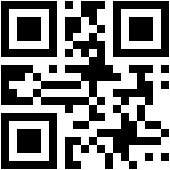
\includegraphics[width=20mm]{images/qrCodeComplex/1}}}
   		 \qquad
		\subfloat[50 encoded characters.]{{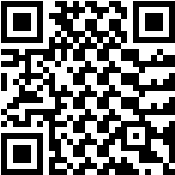
\includegraphics[width=20mm]{images/qrCodeComplex/50}}}
   		 \qquad
		\subfloat[100 encoded characters.]{{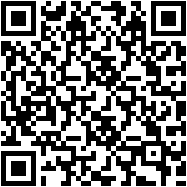
\includegraphics[width=20mm]{images/qrCodeComplex/100}}}
   		 \qquad
		\caption{The three different QR codes used in the complexity test.}
		\label{qrCodeComplex}
	\end{figure}

%	\begin{table}[H]%ht!]
%    		\caption{Average time of registering a QR code with varying density.} \label{tab:complexityAverage}
%		\centering \begin{tabularx}{\textwidth}{l|X|X|X} \hline
%		\textbf{Encoded Characters} & \textbf{Google Glass (sec)} & \textbf{Samsung Galaxy SII (sec)} & \textbf{Samsung Galaxy SIII (sec)} \\ \hline \hline
%       
%		1	&	&	&	\\ \hline
%		50	&	&	&	\\ \hline
%		100	&	&	&	\\ \hline
%		
%		\end{tabularx}
%	\end{table}

\subsubsection{Display Time}

Using the \texttt{Timer} class, seen in Listing~\ref{timerClass}, the elapsed time from the point that the product information had ben downloaded until the information was sent to the display was measured for each device. The test was performed 30 times for each device, with 3 different sizes of product information. Figure~\ref{projectmap} described the application functionality and this test measures steps 4 and 5 in Figure~\ref{projectmap}. The results of the test can be seen in detail in Appendix~\ref{app:results} but will also be presented in a smaller table with the average time. %in a table similar to Table~\ref{tab:averageDisplaySpeedGoogleGlass}. 
Although the \texttt{Timer} class will give the elapsed time in nanoseconds the result will be presented in seconds in order to clearly show the significance of each time as small, nano seconds, differences between devices will not matter as much as seconds.

%	\begin{table}[ht!]
%    		\caption{Average display time for Google Glass with varying information size.} \label{tab:averageDisplaySpeedGoogleGlass}
%		\centering \begin{tabularx}{\textwidth}{l|X|X|X} \hline
%		\textbf{Information Size (Bytes)} & \textbf{Google Glass (sec)}  & \textbf{Samsung Galaxy SII (sec)}  & \textbf{Samsung Galaxy SIII (sec)} \\ \hline \hline
%       
%		1 000		&	&	&	 \\ \hline
%		100 000		&	&	&	 \\ \hline
%		1 000 000		&	&	&	 \\ \hline
%
%		\end{tabularx}
%	\end{table}

\subsection{Summary}
\label{subsec:summary}
The application works in such a way that the first screen the user sees when launching the application, on both Google Glass and smartphones, is the camera screen. The user is then to position the device in such a way that the QR code may be scanned by the device's camera. The QR code contains a product ID for a specific product.

The user does not need to press any shutter button in order to scan the QR code. Instead the application will automatically recognise any QR code pattern that appears in the camera view, as well as scan the QR code. The reason for not implementing a start menu or any similar start screen, to show the user before the camera screen is displayed, is to, according to Google's design guidelines, maintain the focus on what the application is intended to do and to keep the application simple and easy to use.

Next the application will decode the QR code. The decoding process is done by the ZXing library, which is an open source  barcode image processing library. The QR code contains a product ID which is then used in the downloading process. The downloading process entails connecting to a database containing information about different products, and, by using the decoded product ID, retrieving the information on the specific product. 

The downloaded information contains the product name, as well as a list of components and the instructions necessary to assemble the product. All the information is then sorted in to respective classes and the information may be displayed to the user. When the product information is being downloaded a loading animation is displayed on screen. On Google Glass the loading information is a loading bar at the bottom of the screen, and in the smartphone application the loading animation is a spinning wheel.

When the download process has finished the information is displayed to the user in the form of a slide show. The first slide that is displayed to the user is the title slide. The title slide contains the name of the product as well as an image  (if an image existed in the database). Following the title slide are the component slides. Each component has their own slide due to the fact that a component may be described in both text and an image. 

After all the component slides follow the instruction slides. Similar to the components an instruction my be presented by text only or by both text and an image. In contrast to the components, however, instructions may also be presented with an image and no text. 

As Google provides developers of Google Glass applications with predefined layouts, these layouts were also used for the Google Glass application. The layouts used were ``Title'', ``Columns'', ``Text'' and ``Caption''. The predefined layouts were also used as basis for the layouts used in the smartphone application.

The Title layout is used for the title card. The Columns layout is used for the slides with both text and an image. The Text layout is used for the slides with text only. The Caption layout is used for the slides containing only an image. All layouts, except for the Title layout, also contain text at the bottom of the screen called ``footer'' and ``timestamp''. The footer contains information on whether the current slide is a component slide or an instruction slide. The timestamp contains information on which slide is currently being viewed.

While browsing through the slides in the Google Glass application, the user may also navigate using voice commands. The voice commands available in the Google Glass application are ``Show next slide'', ``Show previous slide'', ``Show components'', ``Show instructions'' and ``Scan again''.

Most of the voice commands follow 11 out of the 15 voice command guidelines provided by Google. For example, ``Show components'' does not follow the guidelines which state that ``Is general enough to apply to multiple Glassware, but still has a clear purpose''. ``Show components'' is a specific voice command and could potentially apply to multiple Google Glass applications, but not all.

While viewing the slides ``ok glass'' is shown at the bottom of the screen. ``ok glass'' indicates that voice commands are available and saying ``ok glass'' at that point brings up the voice command menu, showing all available voice commands. However, ``ok glass'' is also shown in combination with a dark, transparent overlay, which ensures ``ok glass'' is always visible no matter what image is shown on screen, but the dark overlay also means that any image shown is darkened by the overlay.

In terms of the testing performed on the application, the experimental setup consisted of an optical bench on which the QR code was positioned at the zero mark, and then each specific device was positioned so that the camera of each device was positioned according to the specifications of each test. Each test result was then obtained through a laptop with which each device was connected via a USB cable. The test results were printed out from a timer class, called \texttt{Timer}, which was implemented using the singleton design pattern, meaning that the class had only one global instance which could be accessed from anywhere within the application.

The test which did not require the experimental setup was the text length test. Instead the text length test was performed using a class which randomised English characters, which were then concatenated together to form a longer string.

Three other tests were performed using the experimental setup. In the first of these three tests the distance to the QR code was varied. In the second test the complexity of the QR code was varied. In the third and final test the size of the downloaded information was varied. Each of these tests were performed 30 times, for each device and each different specification, to ensure statistical significance.

o   Implementation - Present your project implemetion in general
o   Information - Give details here (possibly several sub-sections)
o   Summary - for this chapter

% Mobile phone application
% Uses Zxing - library for QR code scanning [Link to gihub repository missing!!!]
% can display both text and images 
% 
% Google Glass Application
% Uses BarcodeEye - library for QR Code Scanning (port of Zxing for Google Glass) [Link to github repository missing!!!]
% Can display text, images still todo
% Much easier to add slides on Google Glass compared to Mobile Phone Application. Probably because Cards is standard interface for Google Glass (might also be because simple API, check CardPresenter!!!)
% Very difficult to add images since cards can't be changed after .getView() has been called
% Need to call .notifyViewChanged() but does not work anyway (yet) seems to only start the activity over which calls the execute method again if no check has been put in place